%=====================================================================
%  03-LATAR-BELAKANG.TEX
%=====================================================================
\section{LATAR BELAKANG}

\begin{frame}
    \frametitle{Latar Belakang}
    \vspace{-0.5cm}
    \begin{columns}[T]
        \small
        \begin{column}{0.5\textwidth}
            \begin{figure}
                \centering
                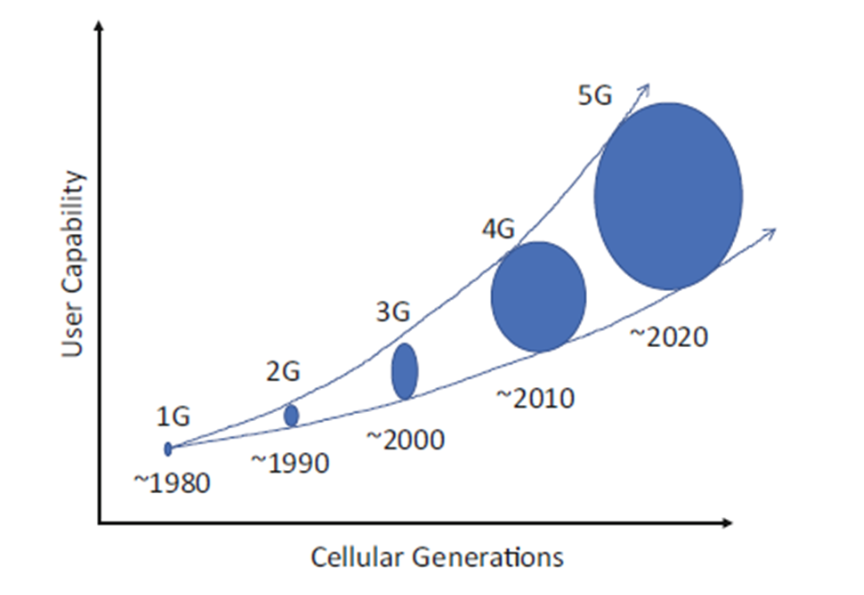
\includegraphics[width=\textwidth]{gambar/BASIC/cellular generation.png}
                \captionsetup{font=tiny, justification=justified, width=\textwidth}
                \captionof{figure}{Perkembangan \textit{user capability}
                berdasarkan \textit{cellular generations}.}
                \label{fig:cellular-generation}
            \end{figure}
        \end{column}

        \begin{column}{0.5\textwidth}
            \begin{itemize}\tiny\justifying
                \item Kemampuan pengguna seluler dengan fitur yang diharapkan
                      berkembang secara eksponensial selama evolusi generasi seluler.
                \item Teknologi komunikasi terus berkembang pesat, mendorong
                      kebutuhan akan akses data yang lebih cepat dan efisien.
                \item Pengguna seluler di Indonesia meningkat 68\% dalam satu
                      dekade terakhir \cite{annur2022kepemilikan}.
                \item Seiring bertambahnya jumlah pengguna seluler, teknik
                      \textit{multiple access} berperan mengatasi keterbatasan
                      sumber daya dan meningkatkan efisiensi saluran komunikasi.
                \item Teknik \textit{multiple access} yang umum: TDMA
                      (\textit{Time Division Multiple Access}), FDMA
                      (\textit{Frequency Division Multiple Access}), CDMA
                      (\textit{Code Division Multiple Access}), dan OFDMA
                      (\textit{Orthogonal Frequency Division Multiple Access}).
                \item Dalam hal kecepatan dan efisiensi, teknologi kuantum dapat
                      dipertimbangkan karena proses komputasinya dilakukan
                      secara paralel.
                \item Pada komputasi kuantum, kriptografi kuantum, dan komunikasi
                      kuantum, \textit{entanglement} berpotensi menyediakan
                      komunikasi yang sangat aman dan efisien.
                \item Penelitian ini menganalisis seberapa potensial
                      \textit{entanglement} diadaptasi ke \textit{multiple
                      access channel} berbasis kuantum.
            \end{itemize}
        \end{column}
    \end{columns}
\end{frame}
